\section{Intoduction}
\begin{frame}
    \begin{definition}
        A signed graph is a graph where each edge is labelled as positive ($+$) or negative ($-$).
    \end{definition}
    \begin{figure}[H]
        \centering
        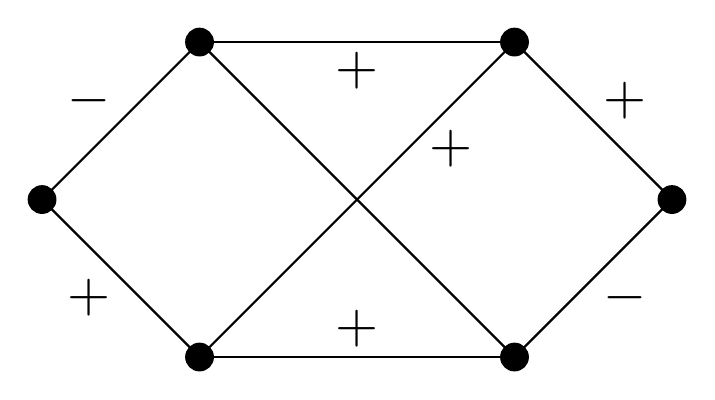
\begin{tikzpicture}[scale=1]
            %graph
            \draw[thick] (2,2)--(4,0);

            \node[right] at (3,1.25) {\(\scalebox{2}{\(+\)}\)};
    
            \draw[thick] (4,0)--(2,-2);

            \node[right] at (3,-1.25) {\(\scalebox{2}{\(-\)}\)};
    
            \draw[thick] (2,-2)--(-2,-2);

            \node[above] at (0,-2) {\(\scalebox{2}{\(+\)}\)};
    
            \draw[thick] (-2,-2)--(-4,0);

            \node[left] at (-3,-1.25) {\(\scalebox{2}{\(+\)}\)};
    
            \draw[thick] (-4,0)--(-2,2);

            \node[left] at (-3,1.25) {\(\scalebox{2}{\(-\)}\)};
    
            \draw[thick] (-2,2)--(2,2);

            \node[below] at (0,2) {\(\scalebox{2}{\(+\)}\)};
    
            \draw[thick] (-2,2)--(2,-2);

            \node[below] at (1.2,1) {\(\scalebox{2}{\(+\)}\)};
    
            \draw[thick] (2,2)--(-2,-2);
    
            \draw[fill] (-2,2) circle (5pt);
    
            \draw[fill] (2,2) circle (5pt);
    
            \draw[fill] (4,0) circle (5pt);
    
            \draw[fill] (2,-2) circle (5pt);
    
            \draw[fill] (-2,-2) circle (5pt);
    
            \draw[fill] (-4,0) circle (5pt);
        \end{tikzpicture}
    \end{figure}
\end{frame}